\chapter{输入输出}\label{ch18}

\emph{Doolittle: What concrete evidence do you have that you exist?
Bomb \#20: Hmmmm... well... I think, therefore I am.
Doolittle: That’s good. That’s very good. But how do you know that anything else exists?
Bomb \#20: My sensory apparatus reveals it to me.}

\begin{flushright}
    ——Dark Star
\end{flushright}

Rust中有关输入输出的特性围绕着三个trait:\texttt{Read}、\texttt{BufRead}、\texttt{Write}来组织:
\begin{enumerate}
    \item 实现了\texttt{Read}的值有读取字节输入的方法。它们被称为\emph{读者(reader)}。
    \item 实现了\texttt{BufRead}的值是\emph{buffered reader(有缓存的读者)}。它们支持\texttt{Read}的所有方法,加上读取文本的一行的方法,等等。
    \item 实现了\texttt{Write}的值支持字节和UTF-8文本输出。它们被称为\emph{写者(writer)}。
\end{enumerate}

\autoref{f18-1}展示了这三个trait以及一些reader和writer类型的示例。

在本章中,我们将解释如何使用这些trait和它们的方法,包括图中出现的reader和writer类型,还有一些其他的和文件、终端、网络交互的方法。

\begin{figure}[htbp]
    \centering
    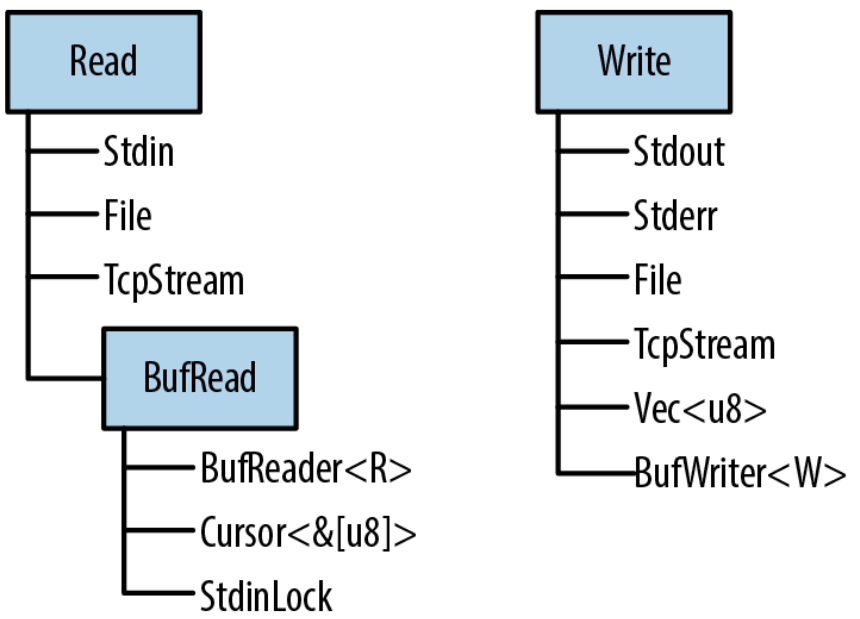
\includegraphics[width=0.8\textwidth]{../img/f18-1.png}
    \caption{Rust的三个主要的I/O trait以及一些实现了它们的类型}
    \label{f18-1}
\end{figure}

\section{Reader和Writer}

\emph{Reader}是你的程序可以从中读取字节的值。例如:
\begin{enumerate}
    \item 使用\texttt{std::fs::File::open(filename)}打开的文件
    \item 用于从网络中接收数据的\texttt{std::net::TcpStream}
    \item 进程用来读取标准输入的\texttt{std::io::stdin()}
    \item \texttt{std::io::Cursor<\&[u8]>}和\texttt{std::io::Cursor<Vec<u8>>}值,它们是从内存中的字节数组或vector中“读取”数据的reader
\end{enumerate}

\emph{Writer}是你的程序可以向其中写入字节的值。例如:
\begin{enumerate}
    \item 使用\texttt{std::fs::File::create(filename)}打开的文件
    \item 用于向网络中发送数据的\texttt{std::net::TcpStream}
    \item 用于写入到终端的\texttt{std::io::stdout()}和\texttt{std::io::stderr()}
    \item \texttt{Vec<u8>},它也是一个writer,它的\texttt{write}方法把数据附加到尾部
    \item std::io::Cursor<Vec<u8>>,类似于上面,但允许你同时读取和写入数据,并可以在vector中定位到不同位置
    \item std::io::Cursor<\&mut [u8]>,和\texttt{std::io::Cursor<Vec<u8>>}很像,除了它不能让缓冲区增长,因为它只是已经存在的字节数组的切片
\end{enumerate}

因为有为reader和writer设计的标准trait(\texttt{std::io::Read}和\texttt{std::io::Write}),所以编写可以处理多种输入输出通道的泛型代码是非常普遍的。例如,这里有一个函数拷贝任意reader中的所有字节到任意writer:
\begin{minted}{Rust}
    use std::io::{self, Read, Write, ErrorKind};

    const DEFAULT_BUF_SIZE: usize = 8 * 1024;

    pub fn copy<R: ?Sized, W: ?Sized>(reader: &mut R, writer: &mut W)
        -> io::Result<u64>
        where R: Read, W: Write
    {
        let mut buf = [0; DEFAULT_BUF_SIZE];
        let mut written = 0;
        loop {
            let len = match reader.read(&mut buf) {
                Ok(0) => return Ok(written),
                Ok(len) => len,
                Err(ref e) if e.kind() == ErrorKind::Interrupted => continue,
                Err(e) => return Err(e),
            };
            writer.write_all(&buf[..len])?;
            written += len as u64;
        }
    }
\end{minted}

这是Rust的标准库中的\texttt{std::io::copy()}的实现。因为它是泛型的,你可以使用它从\texttt{File}中读取数据然后写入到\texttt{TcpStream},或者从\texttt{Stdin}读取,然后写入到内存中的\texttt{Vec<u8>},等等。

如果你看不明白这里的错误处理代码,请复习\hyperref[ch07]{第7章}。我们将在接下来的页面中一直使用\texttt{Result}类型;掌握它的工作原理很重要。

这三个\texttt{std::io}的trait:\texttt{Read}、\texttt{BufRead}、\texttt{Write},以及\texttt{Seek}如此常用,以至于有一个只包含这些trait的\texttt{prelude}模块:
\begin{minted}{Rust}
    use std::io::prelude::*;
\end{minted}

本章中你还会见到它一到两次。我们通常也习惯于导入\texttt{std::io}模块自身:
\begin{minted}{Rust}
    use std::io::{self, Read, Write, ErrorKind};
\end{minted}

这里的\texttt{self}关键字声明了\texttt{io}作为\texttt{std::io}模块的一个别名。这样,\texttt{std::io::Result}和\texttt{std::io::Error}可以用\texttt{io::Result}和\texttt{io::Error}更精确地表示出来,等等。

\subsection{Reader}
\texttt{std::io::Read}有几个方法用于读取数据。所有这些方法都通过\texttt{mut}引用获取self参数。

\codeentry{reader.read(\&mut buffer)}
\hangparagraph{从数据源读取一些字节,并存储到给定的\texttt{buffer}中。\texttt{buffer}参数的类型是\texttt{\&mut [u8]}。它最多读取\texttt{buffer.len()}个字节。}
\hangparagraph{返回类型是\texttt{io::Result<u64>},它是\texttt{Result<u64, io::Error>}的类型别名。当成功时,\texttt{u64}值是读取到的字节数——可能等于或着小于\texttt{buffer.len()},\emph{即使还有更多的数据可以读取}。\texttt{Ok(0)}意味着没有更多的输入可以读取。}
\hangparagraph{当出错时,\texttt{.read()}返回\texttt{Err(err)},其中\texttt{err}是一个\texttt{io::Error}值。\texttt{io::Error}是可打印的,为了便于阅读;对于程序来讲,它有一个\texttt{.kind()}方法返回一个\texttt{io::ErrorKind}类型的错误码。这个枚举的成员有例如\texttt{PermissionDenied}和\texttt{ConnectionReset}的名称。大多数的错误类型都不能被忽略,但有一种错误应该进行特殊处理。\texttt{io::ErrorKind::Interrupted}对应Unix的错误码\texttt{EINTR},它意味着读取过程恰好被一个信号打断。除非你的程序想设计为根据信号做一些聪明的操作,否则它应该简单地重试读取操作。上一节中的\texttt{copy()}的代码,就是一个例子。}
\hangparagraph{如你所见,\texttt{.read()}方法非常底层,甚至直接继承了底层操作系统的怪癖。如果你要为一个新的数据源类型实现\texttt{Read} trait,这会赋予你极大的灵活性。但如果你尝试读取一些数据,就会非常难受。因此,Rust提供了几个更高级的便捷方法。它们都有基于\texttt{.read()}的默认实现。它们都处理了\texttt{ErrorKind::Interrupted},因此你不需要再处理。}

\codeentry{reader.read\_to\_end(\&mut byte\_vec)}
\hangparagraph{读取reader种剩余的所有输入,将读到的数据附加到\texttt{byte\_vec}尾部,\texttt{byte\_vec}是一个\texttt{Vec<u8>}。返回一个\texttt{io::Result<uszie>},表示读取到的字节数。}
\hangparagraph{这个方法读取的数据的大小没有限制,因此不要将它用于不受信任的源。(你可以使用\texttt{.take()}方法施加限制,如后文所述。}

\codeentry{reader.read\_to\_string(\&mut string)}
\hangparagraph{和上面相同,不过把数据附加到给定的\texttt{String}。如果流不是有效的UTF-8,它会返回一个\texttt{ErrorKind::InvalidData}错误。}
\hangparagraph{在一些编程语言中,字节输入和字符输入由不同的类型来处理。如今,UTF-8占据主导地位,Rust承认这一事实标准,并且完全支持UTF-8。其他字符集由开源的\texttt{encoding} crate提供支持。}

\codeentry{reader.read\_exact(\&mut buf)}
\hangparagraph{读取恰好足够的数据来填充给定的缓冲区。参数的类型是\texttt{\&mut [u8]},如果在读取够\texttt{buf.len()}个字节之前reader的数据就已经耗光,那么它会返回一个\texttt{ErrorKind::UnexpectedEof}错误。}

上面这些是\texttt{Read} trait的主要方法。除此之外,还有三个以值获取\texttt{reader}的适配器方法,将它转换为一个迭代器或者一个不同的reader:

\codeentry{reader.bytes()}
\hangparagraph{返回一个输入流的字节的迭代器。item的类型是\texttt{io::Result<u8>},因此每一个字节都需要进行错误检查。另外,它会逐字节调用\texttt{reader.read()},因此如果reader没有缓存的话会非常低效。}

\codeentry{reader.chain(reader2)}
\hangparagraph{返回一个新的reader,首先产生\texttt{reader}的所有输入,然后产生\texttt{reader2}的所有输入。}

\codeentry{reader.take(n)}
\hangparagraph{返回一个新的reader,从和\texttt{reader}相同的数据源读取数据,但最多只读取\texttt{n}个字节。}

没有关闭reader的方法。reader和writer通常实现了\texttt{Drop},因此它们会自动关闭。

\subsection{Buffered Reader}
出于性能考虑,reader和writer可以进行\emph{缓存(buffer)},意思是它们有一块内存(缓冲区)用来存储一些输入或输出数据。这样可以减少系统调用的次数,如\autoref{f18-2}所示。在这个例子中,应用调用\texttt{.read\_line()}方法从\texttt{BufReader}中读取数据,\texttt{BufReader}从操作系统获取更大块的输入。

\begin{figure}[htbp]
    \centering
    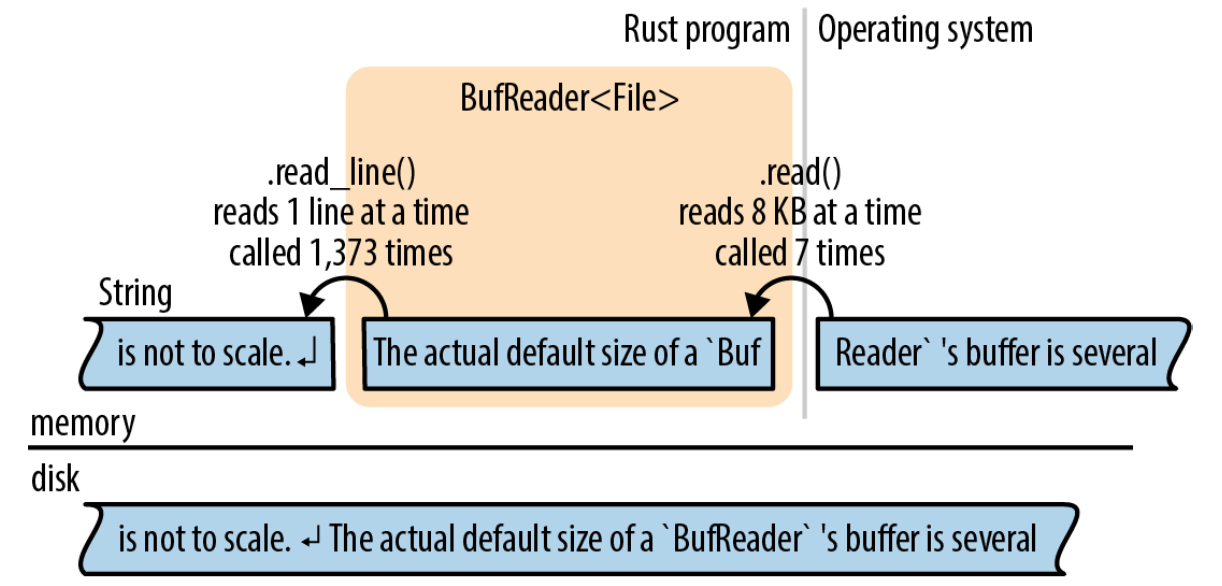
\includegraphics[width=0.9\textwidth]{../img/f18-2.png}
    \caption{一个有缓冲的文件reader}
    \label{f18-2}
\end{figure}

这张图并不是按比例的,一个\texttt{BufReader}的实际大小是几千字节,因此一次系统的\texttt{read}调用可以提供上百次\texttt{.read\_line()}调用。这么做之所以能提高性能是因为系统调用很慢。(如图所示,操作系统也有一个缓冲区,原因与此相同:系统调用很慢,但从磁盘读取数据更慢。)

有缓冲的reader实现了\texttt{Read}和另一个trait \texttt{BufRead},它添加了下面的方法:

\codeentry{reader.read\_line(\&mut line)}
\hangparagraph{读取一行文本并将它附加到\texttt{line},\texttt{line}是一个\texttt{String}。行尾的换行符\texttt{'\\n'}}也会包含在\texttt{line}中。如果输入中有Windows风格的换行符\texttt{"\\r\\n"},这两个字符都会包含进\texttt{line}。
\hangparagraph{返回值是一个\texttt{io::Result<usize>},代表读取到的字节数,包括行尾的换行符。}
\hangparagraph{如果reader到达输入结尾,\texttt{line}会保持不变,并返回\texttt{Ok(0)}。}

\codeentry{reader.lines()}
\hangparagraph{返回一个迭代输入中每一行的迭代器。item的类型是\texttt{io::Result<String>}。换行符\emph{不}包含在字符串中。如果输入中有Windows风格的换行符\texttt{"\\r\\n"},这两个字符都会被丢球。}
\hangparagraph{这个方法几乎总是你需要的文本输入方法。下面的两节会通过例子展示如何使用它。}

\codeentry{reader.read\_until(stop\_byte, \&mut byte\_vec), reader.split(stop\_byte)}
\hangparagraph{这两个方法类似于\texttt{.read\_line()}和\texttt{.lines()},但是是面向字节的,产生\texttt{Vec<u8>}而不是\texttt{String}。你可以选择终止符\texttt{stop\_byte}。}

\texttt{BufRead}还提供两个底层的方法\texttt{.fill\_buf()}和\texttt{.consume(n)},用来直接访问reader的内部缓冲区。更多有关这些方法的信息,可以查阅在线文档。

接下来的两节详细介绍了有缓冲的reader。

\subsection{读取行}\label{ReadLines}
这里有一个实现了Unix \texttt{grep}工具的函数。它搜索文本的每一行,文本通常通过管道从另一个命令输入。对于一个给定的字符串:
\begin{minted}{Rust}
    use std::io;
    use std::io::prelude::*;

    fn grep(target: &str) -> io::Result<()> {
        let stdin = io::stdin();
        for line_result in stdin.lock().lines() {
            let line = line_result?;
            if line.contains(target) {
                println!("{}", line);
            }
        }
        Ok(())
    }
\end{minted}

因为我们想要调用\texttt{.lines()},所以我们需要一个实现了\texttt{BufRead}的输入源。在这个例子中,我们调用了\texttt{io::stdin()}来获取通过管道传入的数据。然而,Rust标准库使用了一个mutex来保护\texttt{stdin},我们调用\texttt{.lock()}来锁住\texttt{stdin}以让当前的线程独占使用,它返回一个实现了\texttt{BufRead}的\texttt{StdinLock}值。在循环的结尾,\texttt{StdinLock}被丢弃,释放mutex。(如果没有mutex,那么如果两个线程同时从\texttt{stdin}中读取数据,会导致未定义行为。C里也有这个问题,它通过这种方式解决它:C中所有的输入和输出函数会在幕后获取一个锁。Rust中唯一的不同就是锁是API的一部分。)

函数的剩余部分非常直观:它调用\texttt{.lines()}并迭代返回的迭代器。因为这个迭代器产生\texttt{Result}值,所以我们使用\texttt{?}操作符来检查错误。

假设我们想进一步扩展我们的\texttt{grep}程序,让它支持搜索磁盘中的文件。我们可以把函数修改为泛型的:
\begin{minted}{Rust}
    fn grep<R>(target: &str, reader: R) -> io::Result<()>
        where R: BufRead
    {
        for line_result in reader.lines() {
            let line = line_result?;
            if line.contains(target) {
                println!("{}", line);
            }
        }
        Ok(())
    }
\end{minted}

现在我们可以向它传递一个\texttt{StdinLock}或者一个有缓存的\texttt{File}:
\begin{minted}{Rust}
    let stdin = io::stdin();
    grep(&target, stdin.lock())?;   // ok

    let f = File::open(file)?;
    grep(&target, BufReader::new(f))?;  // ok
\end{minted}

注意\texttt{File}并不是自动缓存的。\texttt{File}实现了\texttt{Read}但没有实现\texttt{BufRead}。然而,很容易为\texttt{File}或者其他任何无缓存的reader创建一个有缓存的reader。\texttt{BufReader::new(reader)可以实现这个功能。(为了设置缓冲区的大小,可以使用\texttt{BufReader::with\_capacity(size, reader)}。}

在大多数语言中,文件都是默认有缓存的。如果你想要无缓存的输入或输出,你必须知道如何关闭缓存。在Rust中,\texttt{File}和\texttt{BufReader}是两个单独的库特性,因为有时你可能需要没有缓冲的文件,或者需要缓存文件之外的内容(例如,你可能会想要缓存来自网络的输入)。

包含错误处理和一些参数解析的完成的程序,如下所示:
\begin{minted}{Rust}
    // grep - 搜索stdin或文件中匹配给定string的行
    use std::error::Error;
    use std::io::{self, BufReader};
    use std::io::prelude::*;
    use std::fs::File;
    use std::path::PathBuf;

    fn grep<R>(target: &str, reader: R) -> io::Result<()>
        where R: BufRead
    {
        for line_result in reader.lines() {
            let line = line_result?;
            if line.contains(target) {
                println!("{}", line);
            }
        }
        Ok(())
    }

    fn grep_main() -> Result<(), Box<dyn Error>> {
        // 获取命令行参数。第一个参数是要搜索的字符串;
        // 剩余的是文件名。
        let mut args = std::env::args().skip(1);
        let target = match args.next() {
            Some(s) => s,
            None => Err("usage: grep PATTERN FILE...")?
        };
        let files: Vec<PathBuf> = args.map(PathBuf::from).collect();

        if files.is_empty() {
            let stdin = io::stdin();
            grep(&target, stdin.lock())?;
        } else {
            for file in files {
                let f = File::open(file)?;
                grep(&target, BufReader::new(f))?;
            }
        }

        Ok(())
    }

    fn main() {
        let result = grep_main();
        if let Err(err) = result {
            eprintln!("{}", err);
            std::process::exit(1);
        }
    }
\end{minted}

\subsection{收集行}
包括\texttt{.lines()}在内的几个reader方法返回产生\texttt{Result}的迭代器。当你第一次尝试将一个文件的每一行收集到一个很大的vector中时,你可能会遇到需要摆脱\texttt{Result}的问题:
\begin{minted}{Rust}
    // ok,但不是你想要的
    let results: Vec<io::Result<String>> = reader.lines().collect();

    // error: 不能将Result的集合转换成Vec<String>
    let lines: Vec<String> = reader.lines().collect();
\end{minted}

第二次尝试不能编译:哪里出错了?直观的解决方法是编写一个\texttt{for}循环并为每一个item检查错误:
\begin{minted}{Rust}
    let mut lines = vec![];
    for line_result in reader.lines() {
        lines.push(line_result?);
    }
\end{minted}

不错;但这里如果使用\texttt{.collect()}会更好,并且我们确实可以这么做。我们只需要知道需要什么样的类型:
\begin{minted}{Rust}
    let lines = reader.lines().collect::<io::Result<Vec<String>>>()?;
\end{minted}

为什么这能工作?标准库里为\texttt{Result}包含了一个\texttt{FromIterator}的实现——在在线文档中容易忽略——让这变为了可能:
\begin{minted}{Rust}
    impl<T, E, C> FromIterator<Result<T, E>> for Result<C, E>
        where C: FromIterator<T>
    {
        ...
    }
\end{minted}
这个签名需要仔细阅读,但它是一个漂亮的技巧。假设\texttt{C}是任意集合类型,例如\texttt{Vec}或者\texttt{HashSet}。只要我们已经知道了如何从一个产生\texttt{T}值的迭代器构建一个\texttt{C},我们就可以从一个产生\texttt{Result<T, E>}值的迭代器构建一个\texttt{Result<C, E>}。我们只需要遍历迭代器产生的值,用其中的\texttt{Ok}值构建集合,但如何遇到了一个\texttt{Err},就停止并传递它。

换句话说,\texttt{io::Result<Vec<String>>}是一个集合类型,所以\texttt{.collect()}方法可以创建并填充这种类型的值。

\subsection{Writer}
正如我们所见,使用方法就基本可以完成输入。输出有一些不同。

在整本书中,我们都在使用\texttt{println!()}来产生普通文本输出:
\begin{minted}{Rust}
    println!("Hello, world!");

    println!("The greatest common divisor of {:?} is {}", numbers, d);

    println!();     // 打印空白行
\end{minted}

还有一个\texttt{print!()}宏,它不会在最后加上一个换行符,\texttt{eprintln!}和\texttt{eprint!}宏写入到标准错误流。这些函数的格式化代码都和\texttt{format!}宏一样,见“\nameref{format}”。

为了将输出送到一个writer,使用\texttt{write!()}和\texttt{writeln!()}宏。它们与\texttt{print!()}和\texttt{println!()}基本相同,除了两个不同之处:
\begin{minted}{Rust}
    writeln!(io::stderr(), "error: world not helloable")?;

    writeln!(&mut byte_vec, "The greatest common divisor of {:?} is {}", numbers, d)?;
\end{minted}

一个不同之处是\texttt{write}宏有一个额外的第一个参数:writer。另一个不同是它们返回一个\texttt{Result},因此必须进行错误处理。这就是为什么我们在每一行的结尾都使用了\texttt{?}运算符。

\texttt{print}宏不返回一个\texttt{Result},如果写入失败它们会直接panic。因为它们会写入到终端,这是很少见的场景。

\texttt{Write} trait有这些方法:
\codeentry{writer.write(\&buf)}
\hangparagraph{将切片\texttt{buf}中的字节写入到底层的流中。它返回一个\texttt{io::Result<usize>}。成功时,它返回写入的字节数量,可能会小于\texttt{buf.len()},取决于流。}
\hangparagraph{类似于\texttt{Reader::read()},这是一个你应该避免直接使用的底层方法。}

\codeentry{writer.write\_all(\&buf)}
\hangparagraph{写入切片\texttt{buf}中的所有字节。返回\texttt{Result<()>}。}

\codeentry{writer.flush()}
\hangparagraph{冲洗底层流中所有缓存的数据。返回\texttt{Result<()>}。}
\hangparagraph{注意尽管\texttt{println!}和\texttt{eprintln!}宏会自动冲洗标准输出和标准错误流,但\texttt{print!}和\texttt{eprint!}不会。使用它们之后你可能需要手动调用\texttt{flush()}。}

类似于reader,writer也是在丢弃时自动关闭。

类似于\texttt{BufReader::new(reader)}为任意reader添加缓存,\texttt{BufWriter::new(writer)}为任意writer添加缓存:
\begin{minted}{Rust}
    let file = File::create("tmp.txt")?;
    let writer = BufWriter::new(file);
\end{minted}

为了设置缓冲区的大小,使用\texttt{BufWriter::with\_capacity(size, writer)。}

当\texttt{BufWriter}被丢弃时,它剩余的所有被缓存的数据都会被写入到底层的writer。然而,如果这次写入时出现了错误,这个错误会被\emph{忽略}。(因为这个错误是在\texttt{BufWriter}的\texttt{.drop()}方法中发生,没有汇报错误的地方。)为了保证你的应用能够注意到所有的输出错误,可以在drop有缓存的writer之前手动调用\texttt{.flush()}。

\subsection{File}\label{file}
我们已经看到过两种打开文件的方式:
\codeentry{File::open(filename)}
\hangparagraph{打开一个已存在的文件。它返回一个\texttt{io::Result<File>},如果文件不存在将返回一个错误。}

\codeentry{File::create(filename)}
\hangparagraph{创建一个新的文件用于写入。如果已经有同名文件,它会被截断。}

注意\texttt{File}类型在文件系统模块\texttt{std::fs}中,而不是在\texttt{std::io}中。

当这两个文件都不符合要求时,你可以使用\texttt{OpenOptions}来指定额外的期望行为:
\begin{minted}{Rust}
    use std::fs::OpenOptions;

    let log = OpenOptions::new()
        .append(true)   // 如果文件存在,就追加到末尾
        .open("server.log")?;

    let file = OpenOptions::new()
        .write(true)
        .create_new(true)   // 如果文件存在就失败
        .open("new_file.txt")?;
\end{minted}

方法\texttt{.append(), .write(), .create\_new()}等,被设计用来进行类似这样的链式调用:每一个都返回\texttt{self}。这种链式方法的设计模式在Rust中太过普遍以至于有一个专门的名字:它被称为\emph{builder(构建器)}。\texttt{std::process::Command}是另一个例子。更多关于\texttt{OpenOptions}的细节可以查阅在线文档。

\texttt{File}被打开后,它的行为就类似于其他的reader和writer。如果需要的话你可以添加一个缓冲区。当你drop一个\texttt{File}时它会自动关闭。

\subsection{Seek}
\texttt{File}还实现了\texttt{Seek} trait,它意味着你可以在一个\texttt{File}中跳来跳去,而不是只能从开始单调地读到尾。\texttt{Seek}的定义类似如下:
\begin{minted}{Rust}
    pub trait Seek {
        fn seek(&mut self, pos: SeekFrom) -> io::Result<u64>;
    }

    pub enum SeekFrom {
        Start(u64),
        End(i64),
        Current(i64)
    }
\end{minted}

得益于这个枚举,\texttt{seek}方法变得很有表达力:使用\texttt{file.seek(SeekFrom::Start(0))}来定位到开始,使用\texttt{file.seek(SeekFrom::Current(-8))}来回退一些字节,等等。

在一个文件中定位很慢。不管你是在硬盘还是固态盘(SSD)上,定位都要消耗和读取几M数据一样长的时间。

\subsection{其他Reader和Writer类型}
到目前为止,本章中使用了\texttt{File}作为主要的示例,但还有很多其他有用的reader和writer类型:
\codeentry{io::stdin()}
\hangparagraph{返回一个标准输入流的reader。它的类型是\texttt{io::Stdin}。因为它被多个线程共享,所以每一次读取需要请求并释放mutex。}
\hangparagraph{\texttt{Stdin}有一个\texttt{.lock()}方法获取mutex并返回一个\texttt{io::StdinLock},这是一个有缓存的reader,它会持有mutex,直到它被丢弃。因此对\texttt{StdinLock}的单独操作可以避免mutex的开销。我们在“\nameref{ReadLines}”中展示过使用这个方法的示例代码。}
\hangparagraph{出于技术原因,\texttt{io::stdin().lock()}不能工作。这个锁持有一个\texttt{Stdin}值的引用,这意味着\texttt{Stdin}值必须被存储起来,这样它才能生存的足够久:}
\begin{minted}{Rust}
    let stdin = io::stdin();
    let lines = stdin.lock().lines();   // ok
\end{minted}

\codeentry{io::stdout(), io::stderr()}
\hangparagraph{返回标准输出和标准错误流的\texttt{Stdout}和\texttt{Stderr} writer类型。这两个类型也有mutex和\texttt{.lock()}方法。}

\codeentry{Vec<u8>}
\hangparagraph{实现了\texttt{Write}。写入到一个\texttt{Vec<u8>}会把新的数据附加到vector尾部。}
\hangparagraph{然而,\texttt{String}\emph{并没有}实现\texttt{Write}。为了使用\texttt{Write}构建一个字符串,首先要写入到一个\texttt{Vec<u8>},然后使用\texttt{String::from\_utf8(vec)}来把vector转换为字符串。}

\codeentry{Cursor::new(buf)}
\hangparagraph{创建一个\texttt{Cursor},它是一个从\texttt{buf}中读取的有缓存的reader。这也是一个创建从\texttt{String}读取的reader的方法。参数\texttt{buf}可以是任何实现了\texttt{AsRef<[u8]>}的类型,因此你也可以传递一个\texttt{\&[u8], \&str, Vec<u8>}。}
\hangparagraph{Cursor内部的结构非常简单。它只有两个字段:\texttt{buf}和一个整数,用来表示下一次读取开始的偏移量。初始时为0。}
\hangparagraph{Cursor实现了\texttt{Read, BufRead, Seek}。如果\texttt{buf}的类型是\texttt{\&mut [u8]}或\texttt{Vec<u8>},那么\texttt{Cursor}还会实现\texttt{Write}。写入一个Cursor会覆盖\texttt{buf}中从当前位置开始的字节。如果你试图越界写入一个\texttt{\&mut [u8]},结果会是部分写入或者一个\texttt{io::Error}。使用Cursor越界写入一个\texttt{Vec<u8>}没有问题,因为它会让vector变长。因此\texttt{Cursor<\&mut [u8]>}和\texttt{Cursor<Vec<u8>>}实现了\texttt{std::io::prelude}中全部的4个trait。}

\codeentry{std::net::TcpStream}
\hangparagraph{代表一个TCP网络连接。因为TCP允许双向连接,所以它既是reader又是writer。}
\hangparagraph{类型关联函数\texttt{TcpStream::connect(("hostname", PORT))}尝试连接到服务器,并返回一个\texttt{io::Result<TcpStream>}。}

\codeentry{std::process::Command}
\hangparagraph{支持创建一个子进程并把数据管道连接到它的标准输入,例如:}
\begin{minted}{Rust}
    use std::process::{Command, Stdio};

    let mut child =
        Command::new("grep")
         .arg("-e")
         .arg("a.*e.*i.*o.*u")
         .stdin(Stdio::piped())
         .spawn()?;
    
    let mut to_child = child.stdin.take().unwrap();
    for word in my_words {
        writeln!(to_child, "{}", word)?;
    }

    drop(to_child); // 关闭grep的stdin,所以它会退出
    child.wait()?;
\end{minted}
\hangparagraph{\texttt{child.stdin}的类型是\texttt{Option<std::process:ChildStdin>};这里我们在创建子进程的时候使用了\texttt{.stdin(Stdio::piped())},因此当\texttt{.spawn()}成功时\texttt{child.stdin}肯定是\texttt{Some}。否则,\texttt{child.stdin}将是\texttt{None}。}
\hangparagraph{\texttt{Command}还有类似的\texttt{.stdout()}和\texttt{.stderr()}方法,它们可以用来请求\texttt{child.stdout}和\texttt{child.stderr}中的reader。}

\texttt{std::io}模块还提供了很多返回简单reader和writer的函数:
\codeentry{io::sink()}
\hangparagraph{这是一个无操作writer。所有的写入方法都会返回\texttt{Ok},但数据都会被丢弃。}

\codeentry{io::empty()}
\hangparagraph{这是一个无操作reader。所有的读取都会成功,但总是返回输入结束。}

\codeentry{io::repeat(byte)}
\hangparagraph{返回一个无限重复给定字节的reader。}

\subsection{二进制数据,压缩和序列化}
有很多基于\texttt{std::io}框架的开源crate提供额外的特性。

\texttt{byteorder} crate提供\texttt{ReadBytesExt}和\texttt{WriteBytesExt} trait,它们为所有reader和writer添加二进制输入和输出的方法:
\begin{minted}{Rust}
    use byteorder::{ReadBytesExt, WriteBytesExt, LittleEndian};

    let n = reader.read_u32::<LittleEndian>()?;
    writer.write_i64::<LittleEndian>(n as i64)?;
\end{minted}

\texttt{flate2} crate提供读取和写入\texttt{gzip}数据的适配器方法:
\begin{minted}{Rust}
    use flate2::read::GzDecoder;
    let file = File::open("access.log.gz")?;
    let mut gzip_reader = GzDecoder::new(file);
\end{minted}

\texttt{serde} crate,和它的关联的格式化crate例如\texttt{serde\_json},实现了序列化和反序列化:它们在Rust结构体和字节流之间来回转换。我们之前在“\nameref{OrphanRule}”中提到过它们一次。现在让我们仔细看看。

假设我们有一些数据——一个文字冒险游戏的地图——存储在一个\texttt{HashMap}中:
\begin{minted}{Rust}
    type RoomId = String;                       // 每一个房间有一个独一无二的名字
    type RoomExits = Vec<(char, RoomId)>;       // ...和一个通向的房间的名字的列表
    type RoomMap = HashMap<RoomId, RoomExits>;

    // 创建一个简单的地图。
    let mut map = RoomMap::new();
    map.insert("Cobble Crawl".to_string(),
               vec![('W', "Debris Room".to_string())]);
    map.insert("Debris Room".to_string(),
               vec![('E', "Cobble Crawl".to_string()),
                    ('W', "Sloping Canyon".to_string())]);
    ...
\end{minted}

将这个数据转换为JSON并输出只需要一行代码:
\begin{minted}{Rust}
    serde_json::to_writer(&mut std::io::stdout(), &map)?;
\end{minted}

在内部,\texttt{serde\_json::to\_writer}使用了\texttt{serde::Serialize} trait的\texttt{serialize}方法。这个库给所有它知道如何序列化的类型附加了这个trait,其中包括我们的数据中出现的类型:字符串、字符、元组、vector、\texttt{HashMap}。

\texttt{serde}非常灵活。在我们的程序中,输出是JSON数据,因为我们选择了\texttt{serde\_json}序列化器。其他格式例如\texttt{MessagePack}也是可用的。同样地,你可以把输出送到文件、\texttt{Vec<u8>}或其他任何writer中。上面的代码通过\texttt{stdout}打印了数据,内容如下:
\begin{minted}{json}
    {"Debris Room":[["E","Cobble Crawl"],["W","Sloping Canyon"]],"Cobble Crawl": [["W","Debris Room"]]}
\end{minted}

\texttt{serde}还包括派生两个关键trait的支持:
\begin{minted}{Rust}
    #[derive(Serialize, Deserialize)]
    struct Player {
        location: String,
        items: Vec<String>,
        health: u32
    }
\end{minted}

这个\texttt{\#[derive]}属性会让你的编译过程稍微变长,因此当你在\emph{Cargo.toml}文件中将\texttt{serde}作为依赖时需要要求它支持这个特性。这是我们上面的代码用到的依赖:
\begin{minted}{toml}
    [dependencies]
    serde = { version = "1.0", features = ["derive"] }
    serde_json = "1.0"
\end{minted}

更多的细节可以查阅\texttt{serde}的文档。简单来说,构建系统可以自动为\texttt{Player}生成\texttt{serde::Serialize}和\texttt{serde::Deserialize},因此序列化一个\texttt{Player}值非常简单:
\begin{minted}{Rust}
    serde_json::to_writer(&mut std::io::stdout(), &player)?;
\end{minted}

输出看起来是这样的:
\begin{minted}{json}
    {"location":"Cobble Crawl","items":["a wand"],"health":3}
\end{minted}

 
